\documentclass[./main.tex]{subfiles}

\begin{document}
\section{Pretraining}
\label{sec:pretraining}
As we expect our models to require more data than what is in the ClimbAlong dataset to reach their optimal performace, we have decided to pretrain our models on the BRACE and Penn Action datasets, followed by finetuning them on the ClimbAlong dataset. By doing so we expect our models to yield better results than if we were only using the ClimbAlong dataset, as the pretraining-data will be used for adjusting the randomly initialized weights, whereas the finetuning-data will just be used for specializing the model in performancing well on the ClimbAlong dataset. The following section describes the pretraining stage, including the data preprocessing, the used configuration details, as well as the obtained results.
\\
\\
In the pretraining stage we will not be using the already developed pose-estimator, but instead only use our temporal-inclusive models by adding noise to the data such that it simulates the output of the already developed pose-estimator on the ClimbAlong dataset. We do this, as the images of pretraining-data is very different from the ClimbAlong data, making us believe that the already developed pose-estiamtor will yield some very inaccurate results, as well as some predictions that will be very different from the predictions of the model on the ClimbAlong dataset.

\subsection{Data Preprocessing}
As our models take a sequence of estimated poses as input, we will not be using the images of the frames, hence why we discard the images of all frames from BRACE and Penn Action, such that we only keep the annotated poses.
\\
\\
We start by extracting the bounding-box of the annotated pose in each frame by using the annotated keypoints. Further, we expand each side by $10\%$, such that no keypoint lies on any of the boundaries of the bounding-box. To ensure that the aspect ratio of the pose is kept later on, we transform the bounding-box into a square by extending the shorter sides, such that they have the same length as the longer sides. Next, we discard everything outside the bounding-box and rescale the bounding-box to have a sidelength of $56$, such that it has the same size as the output of the already developed pose-estimator.
\\
\\
Next, we transform each frame into twenty five heatmaps. This is done by creating twenty five $56 \times 56$ zero-matrices for each frame, such that each zero-matrix represents a single keypoint of a single frame. Further, for each keypoint we insert a fixed value $c \in \mathbb{R}$ at the position of the keypoint in its corresponding zero-matrix and apply a Gaussian filter with mean $\mu_{out} = 0$ and standard deviation $\sigma_{out} = 1$ to smear out each heatmap. For missing keypoints, we do not place the value $c$ in the corresponding heatmap, making the heatmap consist of only zeros. Further, as Penn Action is the only dataset with the position of the head annotated, as well as the only dataset missing a annotation for the nose, we treat the head-annotation of Penn Action as if it was a nose-annotation, as the position of the two annotation would be very close to each other.
\\
\\
The heatmaps that we produce by following the above description will be used as the groundtruth data. However, as we will be pretraining our models detached from the already developed pose-estimator, we will also need some data as input. We acquire this data by adding some noise to the data, such that they become similar to the output of the already developed pose-estimator, essentially simulating the output of the already developed pose-estimator. The noise is introduced by randomly shifting each keypoint of each sample and by smearing our each keypoint of each sample by using a Gaussian filter with mean $\mu_{in} = 1$ and some standard deviation $\sigma_{in} \in \mathbb{R}_{>0}$. For the shift-value we use $3k$, where the \textbf{shifting-scalar} $k \in \mathbb{R}_{>0}$ is some fixed positive number. We clip the position of the shifted keypoints between $0$ and $55$, such that they cannot be outside of their corresponding heatmaps. 

\subsection{Training Details}
\label{subsubsec:training_details}
\subsubsection{Data Configuration} For the data we use a window-size of $k = 5$ frames, as Artacho \textit{et al.} found this to be the optimal number of frames to use \cite{https://doi.org/10.48550/arxiv.2001.08095}, making our dataset consist of $345,120$ windows. Further, we randomly split our dataset into a training, validation and test set, consisting of $60\%$, $20\%$ and $20\%$ of the data, respectively, without any overlapping or repeating windows among eachother. We insert the fixed value $c = 255$ in each heatmap at the position of the corresponding keypoint. Lastly, to help the models learn the patterns of the data, we shuffle the three subsets, such that the order of which the data is given to the models does not influence the learning.
\\
\\
As the datasets for the pretraining stage are missing some keypoints of the ClimbAlong dataset, we have to cancel out the training of these missing keypoints, as this would otherwise result in the models learning to never predict the presence of these keypoints. There are multiple ways to do this. We handled it during training by setting the groundtruth heatmaps of the missing keypoints equal to the corresponding predicted heatmaps, making the loss of these missing heatmaps be zero and thus the weights of the model of these heatmaps would not be adjusted. 

\subsubsection{Setups} For each of the four models we use three different setups. In the first setup we uniformly at random sample the standard deviation used by the Gaussian filter at the input data $\sigma_{in}$ from the set $\{1, 1.5, 2, 2.5, 3\}$. We do this, as the output heatmaps of the already developed pose-estimator does not use a fixed standard deviation, making the data a better representation of the pose-estimator output. 
\\
\\
As we find it interesting how big of a difference the randomness of the first setup makes, we fix this standard deviation in our second setup, such that we have $\sigma_{in} = 1$, thus, essentially, the models only have to learn to translate the input heatmaps.
\\
\\
Finally, with $30$ frames per second and a window-size of $k = 5$, we suspect that the models might be given too little context to actually be able to effectively smooth out the input data. We could fix this by increasing the window-size, however, we instead chose to make the models work at a lower frame rate, as the increased window-size would also increase the memory usage. Thus, for our last setup we still use a window-size of $5$, however, with half the frame rate. For this setup we also sample $\sigma_{in}$ from the set $\{1, 1.5, 2, 2.5, 3\}$.
\\
\\
As we find it difficult to set the optimal value of the shifting-scalar $k$, such that the data becomes as close as possible to the finetuning data, we run each setup twice for each model. In the first run we use a shifting-scalar of $k = 1$, whereas for the second run we increase this value to $k = 2$, making the data a lot more noisy.

\subsubsection{Training Configuration} For optimizing the weights of the models, we use the ADAM optimizer with a batch size of $16$, an initial learning rate of $10^{-3}$ and the MSE loss-function. During training we keep track of the lowest reached validation loss of an epoch. If this lowest validation loss has not been beaten for five consecutive epochs, we reduce the learning rate by a factor of $0.1$. Further, if the lowest validation loss has not been beaten for ten consecutive epochs, we terminate the training of the corresponding model. In case this never happens, we terminate the training of the corresponding model once it has been trained for fifty epochs.
\\
\\
To reduce the likelihood of vanishing or exploding gradients, we initialize the weights of all models by sampling from the Glorot uniform distribution, defined by
\begin{equation}
    \mathcal{U} \left(- \frac{\sqrt{6}}{\sqrt{n_j + n_{j + 1}}}, \frac{\sqrt{6}}{\sqrt{n_j + n_{j + 1}}} \right),
\end{equation}
where $n_j$ is the size of the previous layer and $n_{j + 1}$ is the size of the layer which is having its weights initialized \cite{glorot2010understanding}.

\subsection{Training and Validation Results}
\begin{figure}[htbp]
    \centering
     \begin{subfigure}[b]{\textwidth}
         \centering
         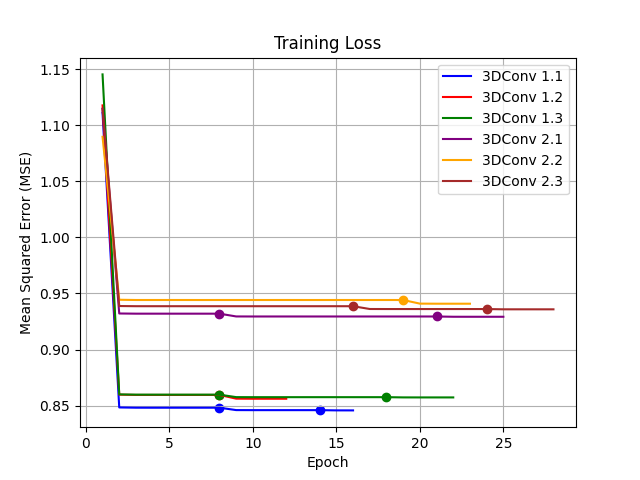
\includegraphics[width=0.32\textwidth]{./entities/pretrained/baseline/train_losses.png}
         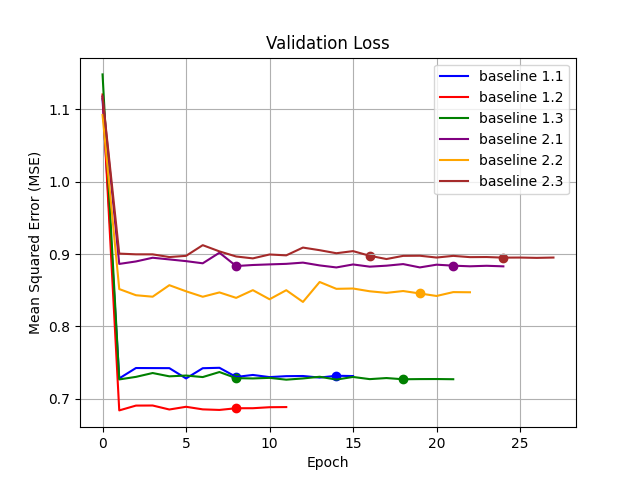
\includegraphics[width=0.32\textwidth]{./entities/pretrained/baseline/val_losses.png}
         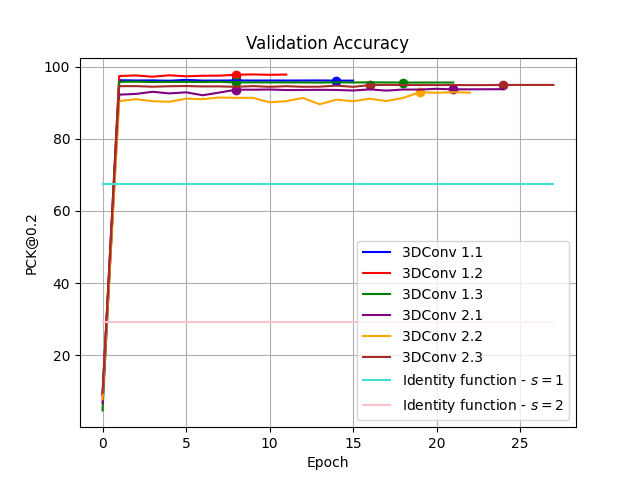
\includegraphics[width=0.32\textwidth]{./entities/pretrained/baseline/val_accs.png}
         \caption{Pretraining results of the 3-dimensional convolutional layer.}
     \end{subfigure}
    \hfill

    \begin{subfigure}[b]{\textwidth}
        \centering
        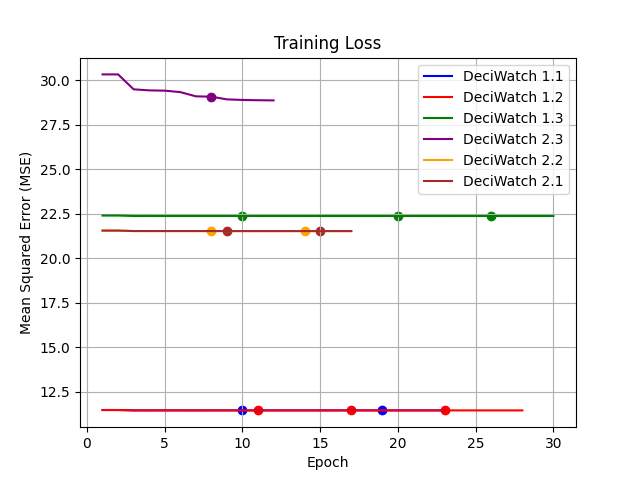
\includegraphics[width=0.32\textwidth]{./entities/pretrained/deciwatch/train_losses.png}
        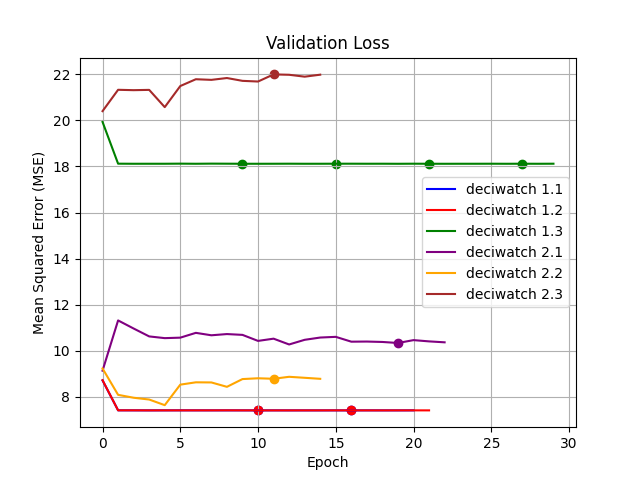
\includegraphics[width=0.32\textwidth]{./entities/pretrained/deciwatch/val_losses.png}
        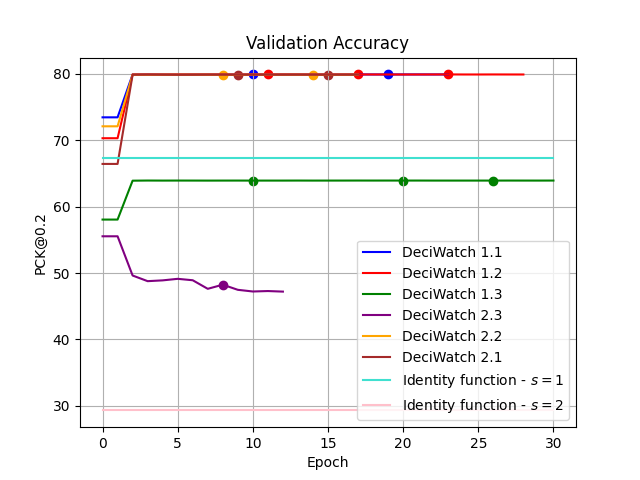
\includegraphics[width=0.32\textwidth]{./entities/pretrained/deciwatch/val_accs.png}
        \caption{Pretraining results of DeciWatch.}
    \end{subfigure}
   \hfill

   \begin{subfigure}[b]{\textwidth}
    \centering
    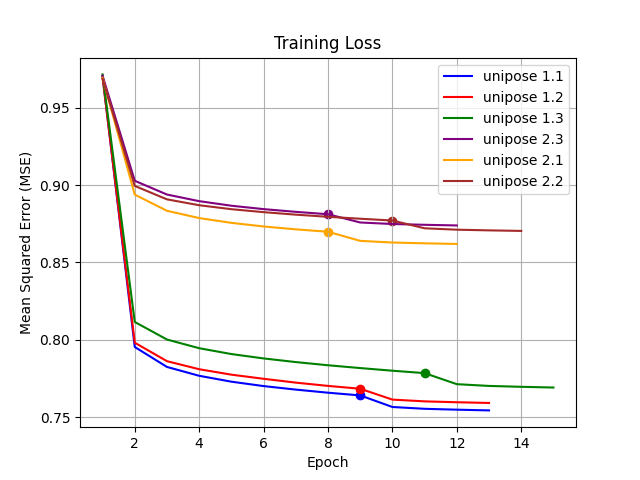
\includegraphics[width=0.32\textwidth]{./entities/pretrained/unipose/train_losses.png}
    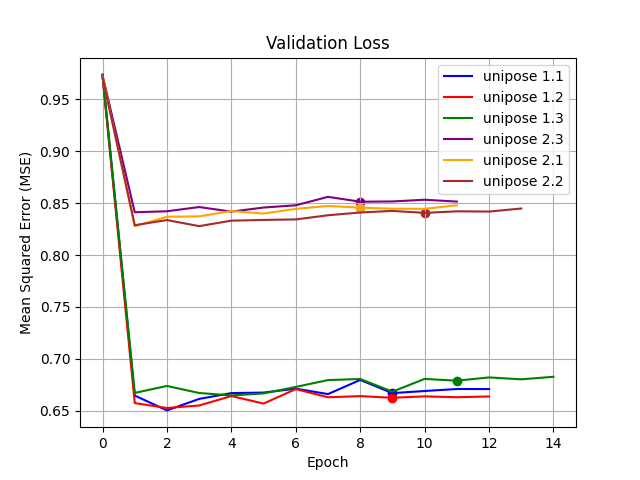
\includegraphics[width=0.32\textwidth]{./entities/pretrained/unipose/val_losses.png}
    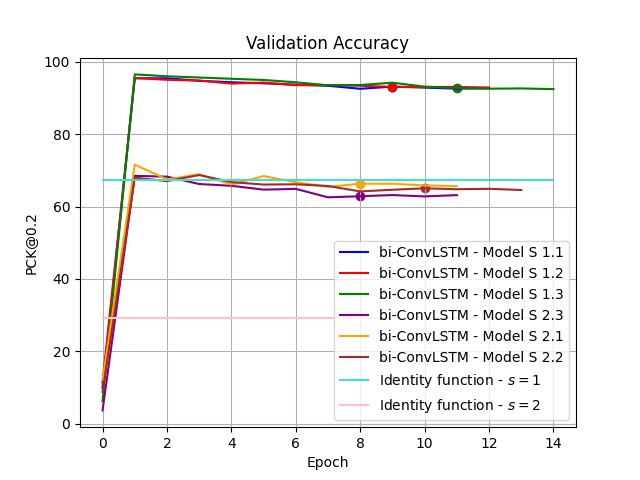
\includegraphics[width=0.32\textwidth]{./entities/pretrained/unipose/val_accs.png}
    \caption{Pretraining results of the bidirectional convolutional LSTM with summing.}
    \end{subfigure}
    \hfill

    \begin{subfigure}[b]{\textwidth}
        \centering
        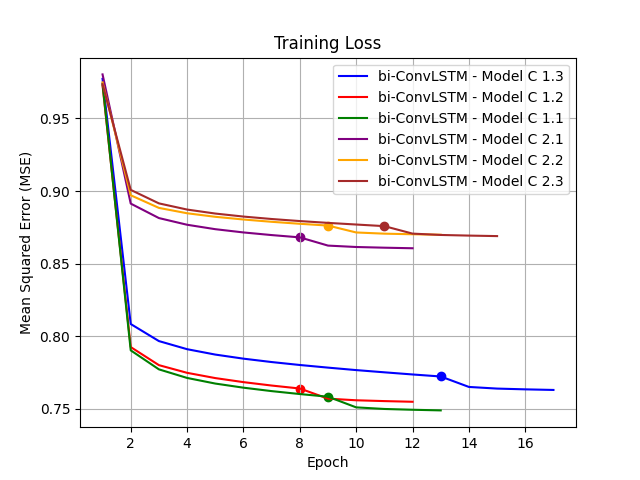
\includegraphics[width=0.32\textwidth]{./entities/pretrained/unipose2/train_losses.png}
        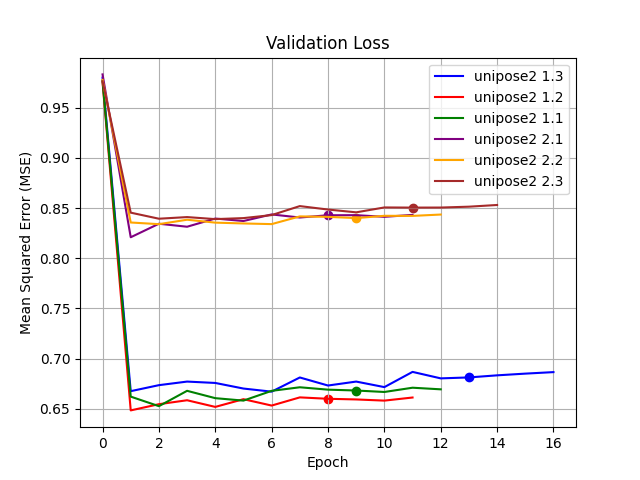
\includegraphics[width=0.32\textwidth]{./entities/pretrained/unipose2/val_losses.png}
        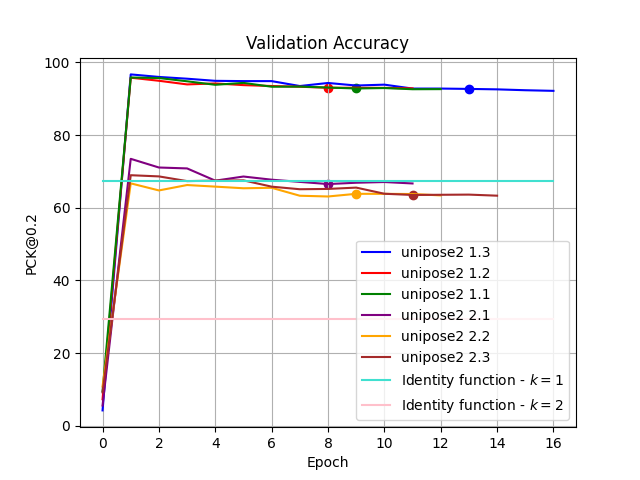
\includegraphics[width=0.32\textwidth]{./entities/pretrained/unipose2/val_accs.png}
        \caption{Pretraining results of the bidirectional convolutional LSTM with concatenation.}
    \end{subfigure}
    \hfill
    
    \caption{Evolution of the training loss, validation loss and validation PCK@0.2 accuracy of the 24 models during training, as well as the validation PCK@0.2 accuracy of the identity function of the two datasets. The dots indicates a reduction of learning-rate. First row: 3-dimensional convolutional layer. Second row: DeciWatch. Third row: Bidirectional Convolutional LSTM with summing. Fourth row: Bidirectional Convolutional LSTM with concatenation.}
    \label{fig:pretrainin_res}
\end{figure}

We have in Figure \ref{fig:pretrainin_res} visualized the evolution of the training loss, validation loss and validation PCK@0.2 accuracy for our 24 models. Each model is delt two numbers seperated by a dot such that it follows a $x.y$-format (for instance, '$2.3$'), indicating what type of experiment and setup it was experimented on. $x$ indicates what shifting-scalar was used when shifting the input keypoints, and $y$ indicates which of the three setups from Section \ref{subsubsec:training_details} the experiment belongs to. Each plot has at least one dot, which indicates the reduction of the learning-rate due to five consecutive epochs without beating the minimum validation loss.
\\
\\
By comparing the validation accuracies of the various models against the identity function we see, that all of the models do learn to somewhat denoise the input data. The simple 3-dimensional convolutional layer seems to be the architecure that generally delivers the greatest results, whereas DeciWatch is generally the architecure that delivers the worst results. Further, the two architectures that are based on bidirectional convolutional LSTMs have close to no difference in their performance, indicating that our raised concern about one of the architectures not being able to prioritize one LSTM-branch over the other is not as great as we hypothesized it to be.
\\
\\
From the figure we can see, that generally the reduction of the learning rate has a pretty substantial effect on the training loss, as the training loss is immediately decreased after a reduction of the learning rate. However, the same cannot be said about the validation loss and accuracy, as these do not immediately decrease after the learning rate has been reduced. Most of the times, the training even terminates before a second reduction of the learning rate takes place, indicating the missing effect of the learning rate reduction on the validation loss and accuracy.
\\
\\
One could look at Figure \ref{fig:pretrainin_res} and argue, that the training of the models generally plateus as soon as after the first epoch, as the evolution of the validation loss and accuracy seems rather flat after the first epoch. However, if we look at when the learning rate reduction happens, we see that more than the five required epochs have passed before the learning rate reduction is taking place, indicating that the learning has not plateued. The evolution of the validation loss and accuracy just seem flat, because the performance difference between the first epoch and the models with their initial weights is so great, that we can have difficuly seeing the performance differences of the following epochs. 
\\
\\
Further, we can clearly see the effects of the shifting-scalar on the training of the models, as all of the models perorms better on the dataset with a low shifting-scalar, than on their corresponding counterpart with a higher shifting-sclar. DeciWatch $1.3$ and DeciWatch $2.3$ do however seems to be struggling quite a bit, as the validation accuracies of these models are much lower than the other DeciWatch models with the same noise-scalar. However, we have to keep in mind here, that DeciWatch already only considers every fifth frame. This, combined with the fact that setup $3$ is only consideren every other frame, makes these two models only consider every tenth frame, which of course makes the prediction very difficult, as these models then have to recover a lot of frames.

\subsection{Test Results}
\begin{table}[htbp]
    \begin{tabular}{c||ccc|ccc|ccc}
        \hline
        Accuracy metric & \multicolumn{3}{c}{PCK@0.05} & \multicolumn{3}{c}{PCK@0.1} & \multicolumn{3}{c}{PCK@0.2} \\
        \hline
        Mean threshold distance* & \multicolumn{3}{c}{1.11} & \multicolumn{3}{c}{2.23} & \multicolumn{3}{c}{4.46} \\
        \hline
        Setup & 1.1 & 1.2 & 1.3 & 1.1 & 1.2 & 1.3 & 1.1 & 1.2 & 1.3 \\
        \hline
        \hline
        Identity function & 6.95 & 6.95 & 6.95 & 25.7 & 25.7 & 25.7 & 67.4 & 67.4 & 67.4 \\
        Conv3D & 1.84 & 20.5 & 0.67 & 30.6 & 58.5 & 23.8 & \textbf{96.6} & \textbf{98.0} & 96.3 \\
        DeciWatch & \textbf{51.4} & \textbf{51.4} & \textbf{44.5} & 64.6 & 64.6 & 51.5 & 80.2 & 80.2 & 64.2 \\
        bi-ConvLSTM - sum. & 27.8 & 31.1 & 33.8 & 68.4 & 71.0 & \textbf{72.5} & 95.7 & 95.8 & 96.7\\
        bi-ConvLSTM - concat. & 29.5 & 31.7 & 31.8 & \textbf{69.5} & \textbf{71.3} & 71.8 & 96.1 & 96.1 & \textbf{96.9} \\
        \hline
    \end{tabular}
    \caption{Testing accuracies of the various developed models for shifting-scalar $k = 1$. All the accuracies are in percentage. *: The mean maximum distance between the predicted keypoint and corresponding groundtruth keypoint for the prediction to count as being correct, using the units of the heatmap coordinates.}
    \label{tab:pretrain_test_accs_1}
\end{table}

\begin{table}[htbp]
    \begin{tabular}{c||ccc|ccc|ccc}
        \hline
        Accuracy metric & \multicolumn{3}{c}{PCK@0.05} & \multicolumn{3}{c}{PCK@0.1} & \multicolumn{3}{c}{PCK@0.2} \\
        \hline
        Mean threshold distance* & \multicolumn{3}{c}{1.11} & \multicolumn{3}{c}{2.23} & \multicolumn{3}{c}{4.46} \\
        \hline
        Setup & 2.1 & 2.2 & 2.3 & 2.1 & 2.2 & 2.3 & 2.1 & 2.2 & 2.3 \\
        \hline
        \hline
        Identity function & 1.84 & 1.84 & 1.84 & 7.75 & 7.75 & 7.75 & 29.3 & 29.3 & 29.3 \\
        Conv3D & 0.80 & 2.40 & 0.11 & 21.6 & 27.6 & 16.8 & \textbf{94.2} & \textbf{91.8} & \textbf{95.5} \\
        DeciWatch & 8.55 & \textbf{35.6} & 8.73 & 27.7 & \textbf{54.8} & 22.1 & 62.7 & 78.4 & 48.0 \\
        bi-ConvLSTM - sum. & 10.5 & 11.6 & \textbf{10.1} & 31.1 & 33.4 & 29.5 & 68.5 & 67.8 & 69.6 \\
        bi-ConvLSTM - concat. & \textbf{12.5} & 12.0 & 9.63 & \textbf{36.4} & 32.5 & \textbf{29.8} & 74.6 & 65.5 & 70.0 \\
        \hline
    \end{tabular}
    \caption{Testing accuracies of the various developed models for shifting-scalar $k = 2$. All the accuracies are in percentage. *: The mean maximum distance between the predicted keypoint and corresponding groundtruth keypoint for the prediction to count as being correct, using the units of the heatmap coordinates.}
    \label{tab:pretrain_test_accs_2}
\end{table}

\noindent We have in Table \ref{tab:pretrain_test_accs_1} and Table \ref{tab:pretrain_test_accs_2} illustrated the test results of the various models on the testsets for PCK$@0.05$, PCK$@0.1$ and PCK$@0.2$.
\\
\\
For shifting-scalar $k = 1$ we see, that DeciWatch is the architecure that yields the best results for PCK$@0.05$ and PCK$@0.1$. However, for PCK$@0.2$ DeciWatch actually tends to be the worst performing model, which means that most of the predicitons of DeciWatch that are considered correct, are actually very close to the groundtruth, whereas the predictions that are incorrect are pretty far off.
\\
\\
On the other hand, the simple 3-dimensional convolutional layer seems to be the architecture that generally performs the worst for PCK$@0.05$ and PCK$@0.1$ and actually the architecture that performs the best for PCK$@0.2$. Thus, the 3-dimensional convolutional layer is very good at inferencing a rough estimate of the position of the keypoints, however, the exact position of these predictions are generally incorrect.
\\
\\
Generally, the bidirectional convolutional LSTMs yield some decent results, as the predicitons of these models are always pretty far away from the worst-performing model for any of the three used accuracy metrics. Similarly to the validation results, the test results do not indicate any major performance differences between the two different types of bidirectional convolutional LSTMs. Likewise, similarly to the validation results, the test results indicate a major effect of a low frame rate for DeciWatch. 
\\
\\
If we take a closer look at the four types of architectures we see, that the 3-dimensional convolutional layer generally performs much better on the second setup that it does on the two other setups. As the models of the first and third setup have to learn both translation and scaling, where for the second setup the model only has to learn translation, we can clearly see how big of an impact the task of scaling the data has for this simple model. As for comparison, the performances of the other architectures have generally a lot smaller variance, indicating these models being less impacted by the setup. This is especially visible for DeciWatch, which has no performance differences between the two first setups. However, this is due the architecture working on keypoint-coordinates instead of heatmaps, making it scaling invariant and thus making it, such that there are no differences between the two first setups.
\\
\\
The testing results of shifting-scalar $k = 2$ generally follow the same pattern with some minor differences. In this case, the bidirectioanl convolutional LSTM with summing is actually the model that yields the best results for PCK$@0.05$ and PCK$@0.1$ instead of DeciWatch, as it was in the case for $k = 1$. However, DeciWatch does still yied some results that are pretty close to the results of the convolutional LSTM with summing.
\\
\\
Unsurprisingly, all of the models performed worse as the shifting-noise was double. Nonetheless, the 3-dimensional convolutional layer is still the architecture that yields the best results when considering PCK$@0.2$. However, unlike the previous case, this architecure now completely outperforms the three alternative architectures, when considering PCK$@0.2$, but is on the other hand completely outperformed by the other models when considering PCK$@0.05$. This indicates, that the architecture can still yield decent rough estimations of the keypoints when a lot of noise is added, however, it does also indicate, that the exact position of these keypoints are very much effected by the level of noise.
\\
\\
Which architecture is the best at denoising the data depends on one's needs. If one just need a rough estimate of the position of the keypoints, then the 3-dimensional convolutional layer would be the optimal choice, as this model has the highest PCK$@0.2$-values. However, if one need the model which yields the most exact predictions, then one of the bidirectional convolutional LSTMs would be the optimal choice.
\\
\\
We have further in Table \ref{tab:pretrain_kpts_test_accs_1} and Table \ref{tab:pretrain_kpts_test_accs_2} illustrated the keypoint-specific testing PCK$@0.2$ of the various models.
\begin{itemize}
    \item $k = 1$
    \begin{itemize}
        \item Wrist og ankle er de dårligste
        \item Ears and Shoulders er de bedste
    \end{itemize}
    \item $k = 2$
    \begin{itemize}
        \item Elbow og knee er de dårligste
        \item Ears and shoulders er de bedste
    \end{itemize}
\end{itemize}

\begin{table}[htbp]
    \begin{adjustbox}{center}
        \begin{tabular}{c||ccc|ccc|ccc|ccc|c}
            \hline
            & \multicolumn{3}{c}{Conv3D} & \multicolumn{3}{c}{DeciWatch} & \multicolumn{3}{c}{\begin{tabular}[c]{@{}c@{}}bi-ConvLSTM\\ sum.\end{tabular}} & \multicolumn{3}{c}{\begin{tabular}[c]{@{}c@{}}bi-ConvLSTM\\ concat.\end{tabular}} & Total \\ 
            \hline
            Setup & 1.1 & 1.2 & 1.3 & 1.1 & 1.2 & 1.3 & 1.1 & 1.2 & 1.3 & 1.1 & 1.2 & 1.3 & \\
            \hline
            \hline
            Nose & 96.2 & 97.3 & 96.3 & 83.0 & 83.0 & 68.0 & 97.3 & 94.2 & 97.8 & 96.2 & 96.4 & 95.9 & \\
            Ear & 96.3 & 97.0 & 96.3 & 85.1 & 85.1 & 69.9 & 96.8 & 96.3 & 96.9 & 96.3 & 96.4 & 96.1 & \\
            Shoulder & 96.7 & 98.6 & 96.7 & 83.8 & 83.8 & 68.6 & 97.0 & 96.9 & 96.0 & 96.5 & 97.0 & 97.2 & \\
            Elbow & 96.7 & 98.7 & 96.4 & 78.3 & 78.3 & 61.8 & 96.1 & 97.6 & 97.6 & 96.1 & 96.5 & 98.5 & \\
            Wrist & 96.5 & 97.8 & 96.2 & 74.0 & 74.0 & 57.7 & 95.8 & 95.0 & 96.2 & 95.9 & 95.5 & 97.0 & \\
            Hip & 96.8 & 99.1 & 96.3 & 80.3 & 80.3 & 64.0 & 93.5 & 95.7 & 96.6 & 96.8 & 95.3 & 96.3 & \\
            Knee & 96.8 & 98.5 & 96.4 & 75.9 & 75.9 & 60.0 & 95.2 & 96.0 & 96.7 & 95.4 & 96.4 & 97.6 & \\
            Ankle & 96.2 & 96.9 & 95.8 & 72.8 & 72.8 & 57.9 & 95.1 & 94.1 & 96.7 & 95.7 & 95.6 & 96.4 & \\
            \hline
        \end{tabular}
        \caption{Keypoint-specific testing PCK@0.2-accuracies of the various models for shiting-scalar $k = 1$. All the accuracies are in percentage.}
        \label{tab:pretrain_kpts_test_accs_1}
    \end{adjustbox}
\end{table}

\begin{table}[htbp]
    \begin{adjustbox}{center}
        \begin{tabular}{c||ccc|ccc|ccc|ccc|c}
            \hline
            & \multicolumn{3}{c}{Conv3D} & \multicolumn{3}{c}{DeciWatch} & \multicolumn{3}{c}{\begin{tabular}[c]{@{}c@{}}bi-ConvLSTM\\ sum.\end{tabular}} & \multicolumn{3}{c}{\begin{tabular}[c]{@{}c@{}}bi-ConvLSTM\\ concat.\end{tabular}} & Total \\ 
            \hline
            Setup & 2.1 & 2.2 & 2.3 & 2.1 & 2.2 & 2.3 & 2.1 & 2.2 & 2.3 & 2.1 & 2.2 & 2.3 & \\
            \hline
            \hline
            Nose & 92.5 & 84.5 & 94.4 & 64.9 & 82.7 & 47.9 & 75.8 & 70.6 & 73.5 & 73.9 & 72.2 & 73.7 & \\
            Ear & 92.0 & 91.1 & 94.4 & 72.5 & 84.7 & 43.9 & 80.3 & 77.7 & 77.7 & 80.8 & 79.2 & 79.9 & \\
            Shoulder & 93.7 & 91.9 & 95.6 & 65.4 & 79.9 & 43.7 & 74.7 & 68.2 & 68.9 & 70.4 & 68.1 & 68.3 & \\
            Elbow & 94.8 & 92.3 & 95.8 & 57.1 & 77.7 & 33.4 & 58.2 & 66.7 & 64.7 & 67.0 & 61.6 & 63.3 & \\
            Wrist & 94.8 & 92.6 & 96.0 & 60.5 & 73.9 & 54.7 & 69.4 & 66.3 & 69.4 & 75.6 & 65.4 & 69.4 & \\
            Hip & 94.5 & 91.6 & 95.7 & 62.4 & 72.4 & 44.9 & 64.7 & 61.9 & 67.5 & 80.7 & 57.3 & 74.8 & \\
            Knee & 95.0 & 92.7 & 95.7 & 53.0 & 75.7 & 51.8 & 60.1 & 65.9 & 64.7 & 68.6 & 57.0 & 54.5 & \\
            Ankle & 95.2 & 94.1 & 95.6 & 59.9 & 72.7 & 57.6 & 69.4 & 67.3 & 72.5 & 78.1 & 67.5 & 77.5 & \\
            \hline
        \end{tabular}
        \caption{Keypoint-specific testing PCK@0.2-accuracies of the various models for shiting-scalar $k = 2$. All the accuracies are in percentage.}
        \label{tab:pretrain_kpts_test_accs_2}
    \end{adjustbox}
\end{table}

\section{Technical Details}

\end{document}